\documentclass[a3paper, 11pt]{article}

\usepackage[T2A]{fontenc}
\usepackage[utf8]{inputenc}
\usepackage[english, russian]{babel}
\usepackage[top=2cm, bottom=2cm, right=2cm, left=2cm]{geometry}
\usepackage{amsmath}
\usepackage{graphicx}
\usepackage{subcaption}
\usepackage{float}
\usepackage{tabularx}

\begin{document}

\section*{Цель работы}
Исследование свойст систем управления.
\section*{Исходные данные}
\begin{center}
    \begin{tabular}{|c|c|c|c|c|c|c|c|}
    \hline
    $W(s)$ & $g = A$ & $g = Vt$ & $g = at^2/2$ & Вариант схемы & $f_1$ & $f_2$ & Сигнал задания \\  \hline
    $\aligned \frac{1.5}{0.5s + 1} \endaligned$ & 2 & 4t & $0.2t^2$ & a) & -0.5 & 1 & $0.5t + 2\cos{(0.1t)}$  \\
    \hline
\end{tabular}
\end{center}

\section*{Исследование системы с астатизмом нулевого порядка.}

\paragraph{Исследование стационарного режима работы: $g(t) = 2$.}
На рисунке 1 представлена диаграмма модели при входном воздействии g = 2, а также полученные графики (рисунок 2) при различных значениях $H(s) = k$. \par
\begin{figure}[H]
    \centering
    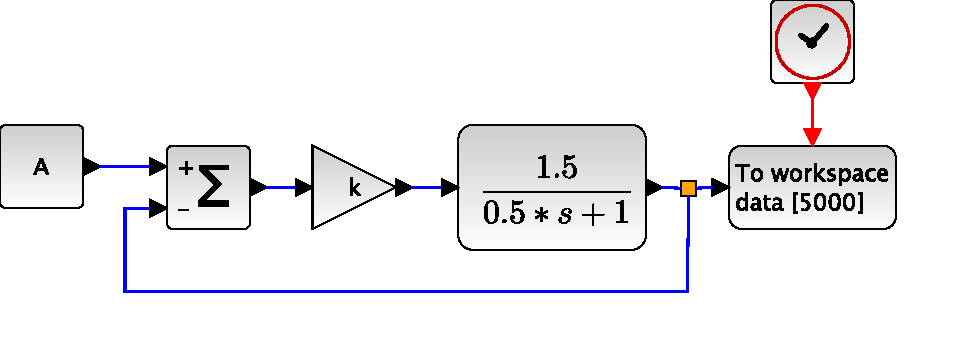
\includegraphics[width = 0.5\textwidth]{images/model1.pdf}
    \caption{Схема моделирования.}
\end{figure}
\begin{figure}[h!]
    \centering
    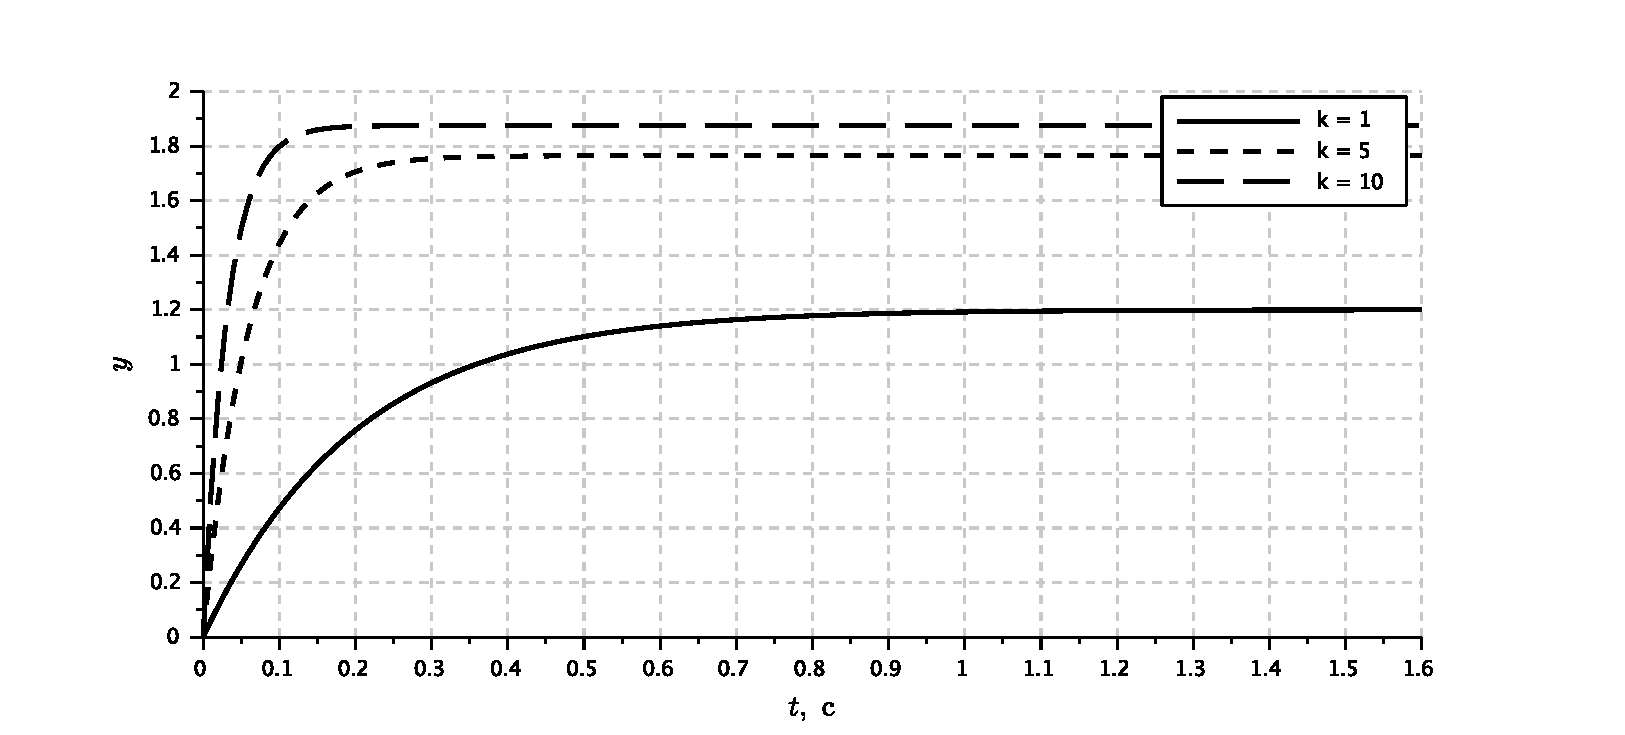
\includegraphics[width = \textwidth]{images/graph1-1.pdf}
    \caption{Графики при различных k.}
\end{figure}

Передаточную функцию ошибки можно представить следующим выражением: 
\begin{equation}
    \Phi_e(s) = \frac{0.5s + 1}{0.5s + 1 + 1.5k}     
\end{equation}
Соответственно можем получить предельное значение ошибки при различных k:
\begin{equation}
    \varepsilon = \lim_{s\rightarrow 0}{\Phi_e(s)}g = \frac{2}{2 + 3k}g
\end{equation}
\begin{align*}
    \varepsilon|_{k = 1} & = 0.8 & \varepsilon|_{k = 5} & \approx 0.235 & \varepsilon|_{k = 10} & = 0.125
\end{align*}


\newpage
\paragraph{Исследование режима работы с постоянной скоростью: $g(t) = 4t$.}
Далее на рисунках 3 и 4 представлены модель и графики моделирования исходной системы при постоянной скорости.
\begin{figure}[h!]
    \centering
    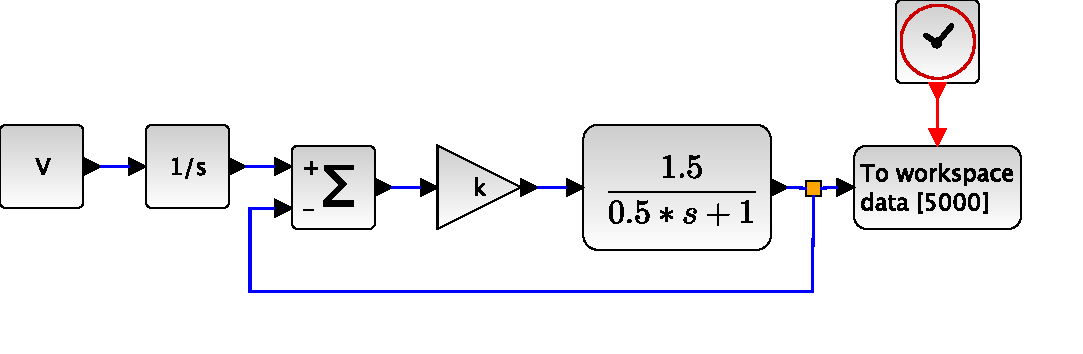
\includegraphics[width = 0.5\textwidth]{images/model1-2.pdf}
    \caption{Схема моделированя.}
\end{figure}
\begin{figure}[h!]
    \centering
    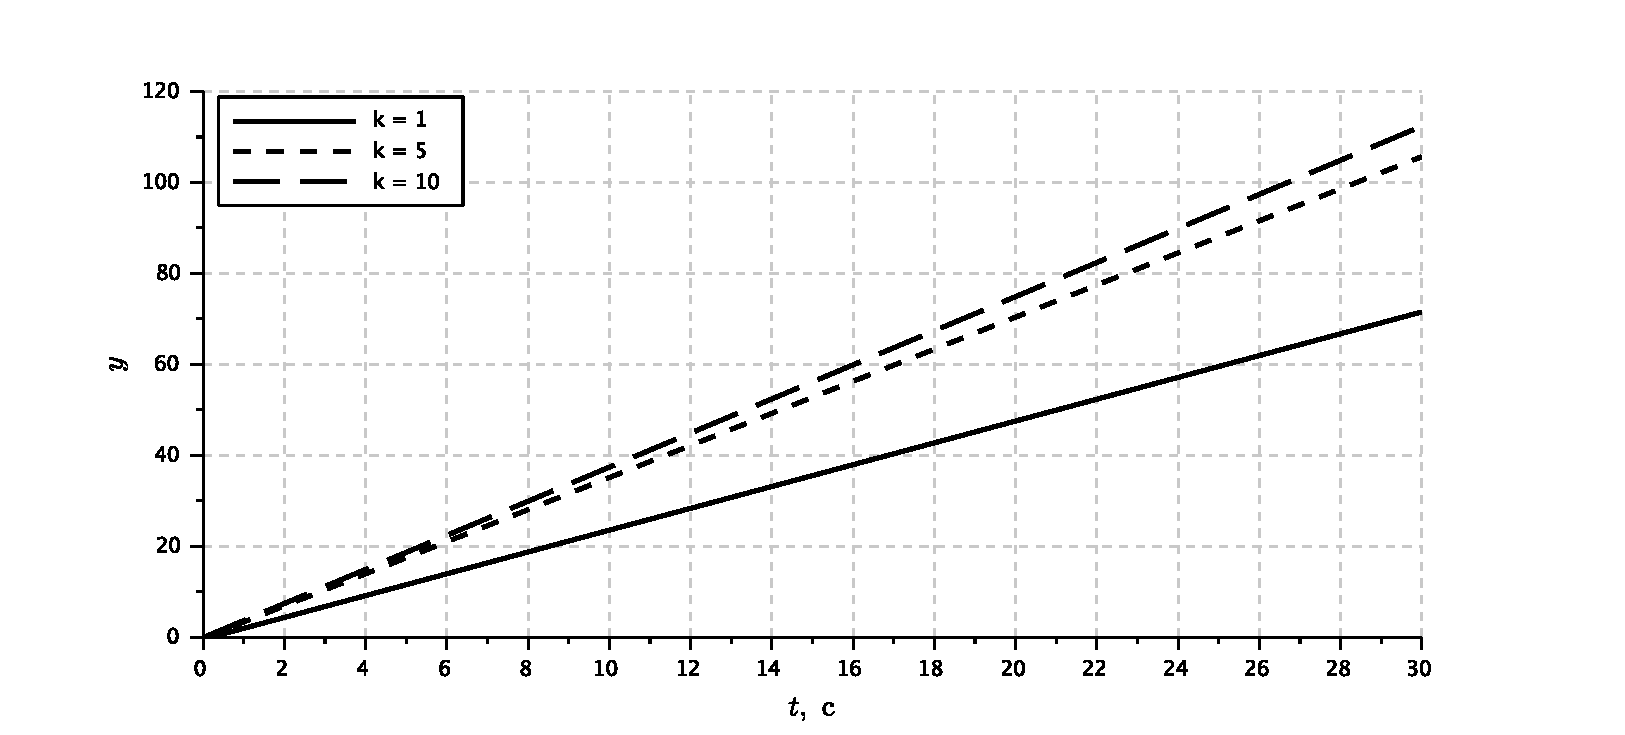
\includegraphics[width = 0.8\textwidth]{images/graph1-2.pdf}
    \caption{График при различных k.}
\end{figure}

\section*{Исследование системы с астатизмом первого порядка.}
\paragraph{Исследование стационарного режима работы: $g(t) = 2$.} На рисунках 5 и 6 представлены диаграмма модели и соответственно полученные графики при различных k.

\begin{minipage}[t]{0.5\textwidth}
    \begin{figure}[H]
        \centering
        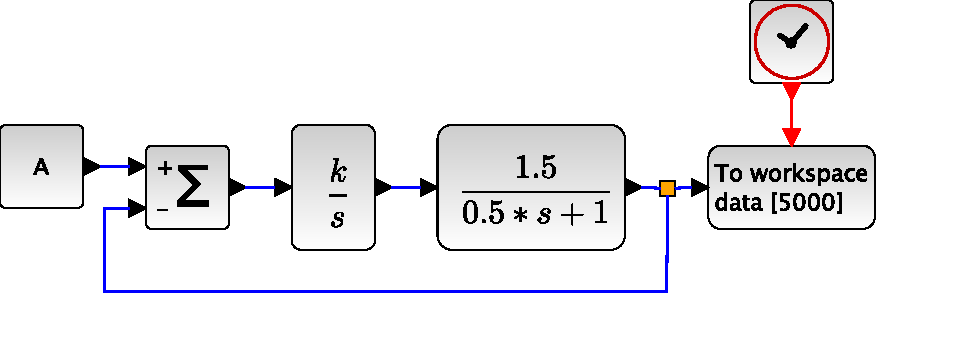
\includegraphics[width = 0.9\textwidth]{images/model2-1.pdf}
        \caption{Схема моделирования.}
    \end{figure}
\end{minipage}
\begin{minipage}[t]{0.5\textwidth}
    \vspace{0.5cm}
    Передаточная функция ошибки:
    \begin{equation}
        \Phi_e = \frac{0.5s^2 + s}{0.5s^2 + s + 1.5k}
    \end{equation}
    Предельное значение ошибки при различных k:
    \begin{equation*}
        \varepsilon = 0;
    \end{equation*}
\end{minipage}

\begin{figure}[h!]
    \centering
    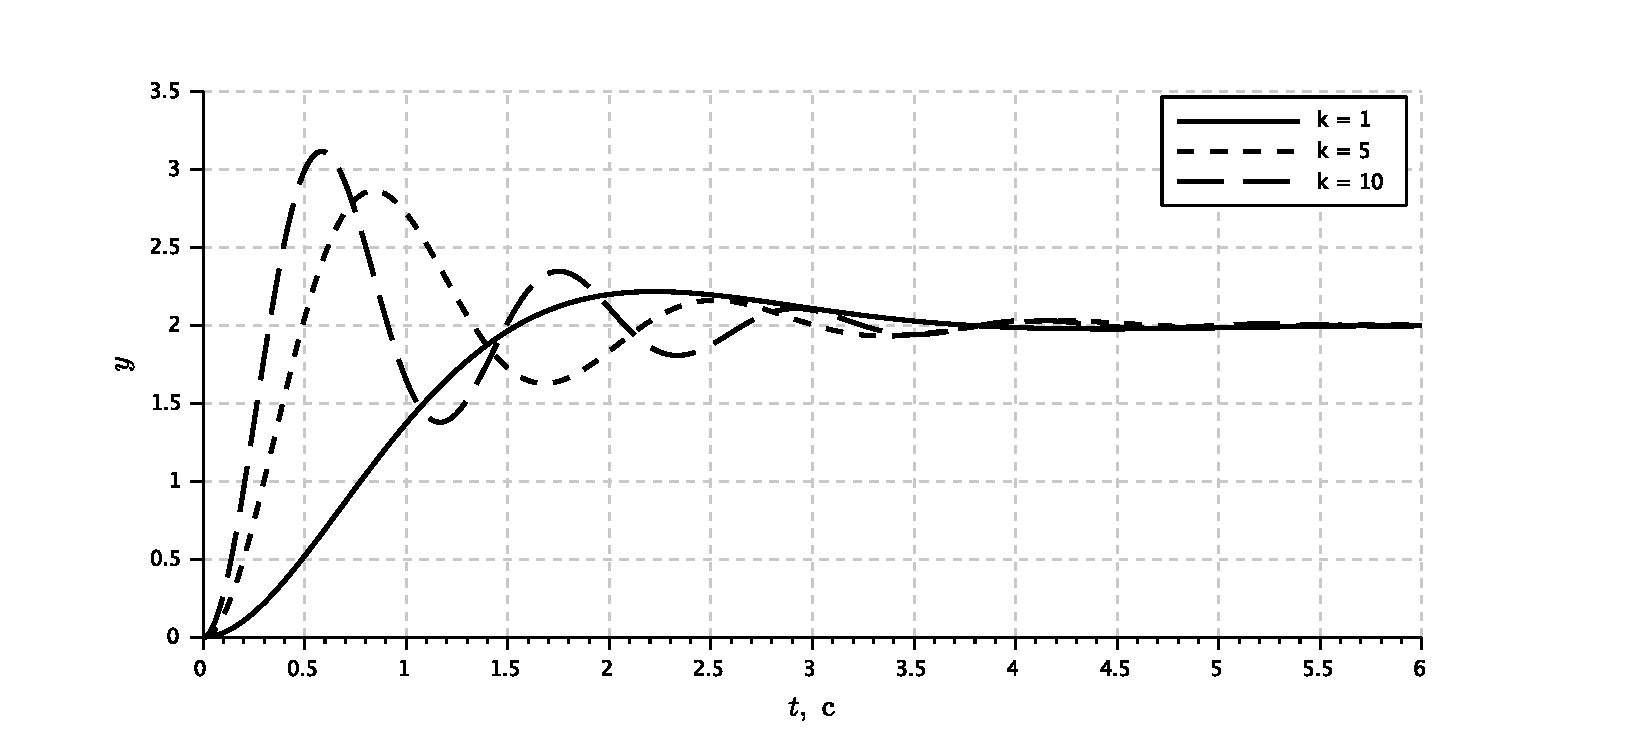
\includegraphics[width = 0.8\textwidth]{images/graph2-1.pdf}
    \caption{Графики при различных k.}
\end{figure}

\paragraph{Исследование режима движения с постоянной скростью: $g(t) = 4t$.} На рисунках 7 и 8 представлены диаграмма модели и соответственно полученные графики при различных k.

\begin{minipage}[t]{0.5\textwidth}
    \begin{figure}[H]
        \centering
        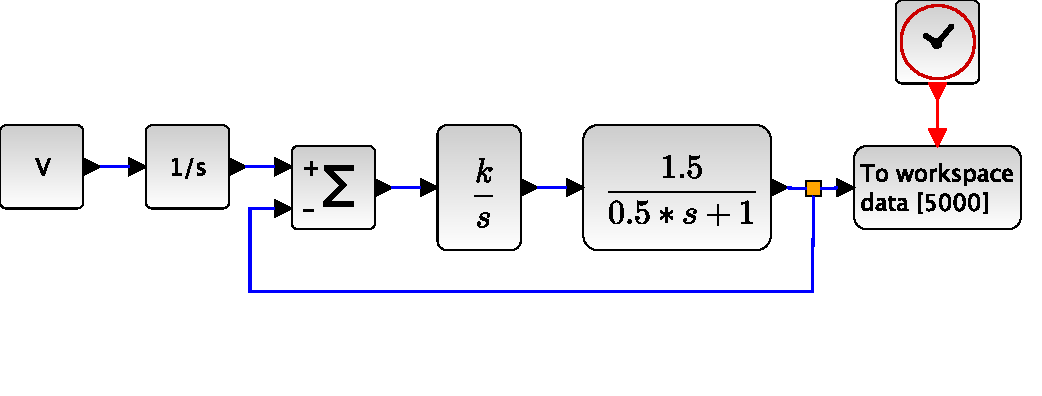
\includegraphics[width = 0.9\textwidth]{images/model2-2.pdf}
        \caption{Схема моделирования.}
    \end{figure}
\end{minipage}
\begin{minipage}[t]{0.5\textwidth}
    \vspace{0.5cm}
    Передаточная функция ошибки представлена в выражении (3).
    Предельное значение ошибки можно записать уравнением:
    \begin{equation}
        \varepsilon = \lim_{s\rightarrow 0}{\Phi_e(s)\frac{4}{s}} = \frac{8}{3k}
    \end{equation}
    Теперь можем получить прдельные значения ошибки при различных k:
    \begin{align*}
        \varepsilon|_{k = 1} & \approx 2.67 & \varepsilon|_{k = 5} & \approx 0.53 & \varepsilon|_{k = 10} & \approx 0.27
    \end{align*}
\end{minipage}

\begin{figure}[h!]
    \centering
    \begin{subfigure}{0.33\textwidth}
        \centering
        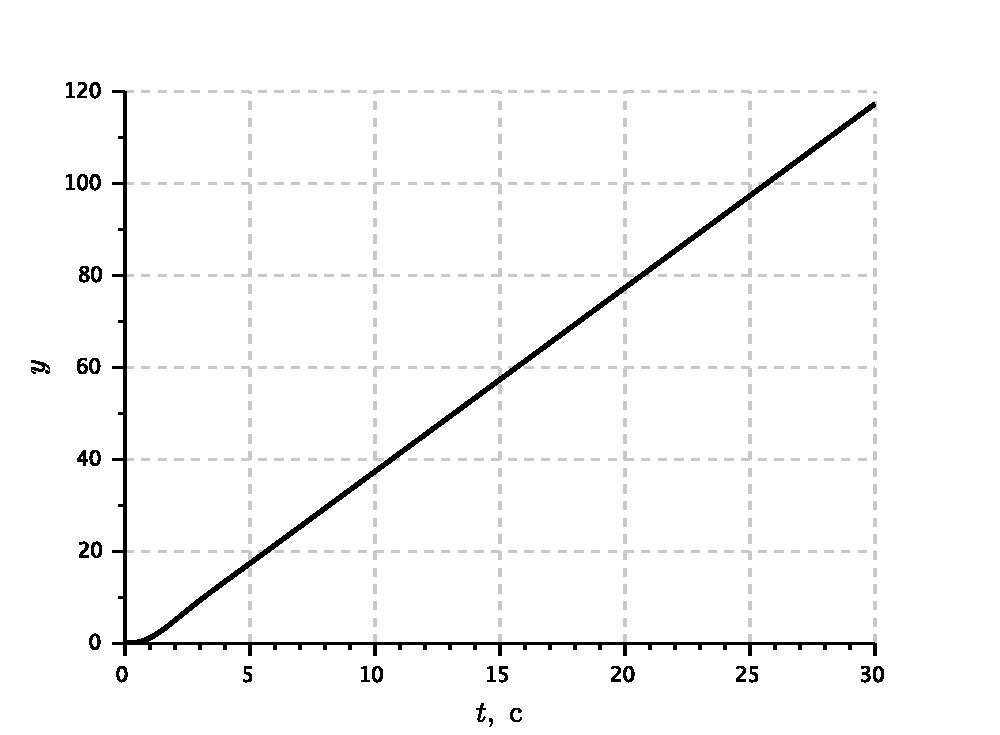
\includegraphics[width = \textwidth]{images/graph2-2-K1.pdf}
        \caption{k = 1}
    \end{subfigure}
    \begin{subfigure}{0.33\textwidth}
        \centering
        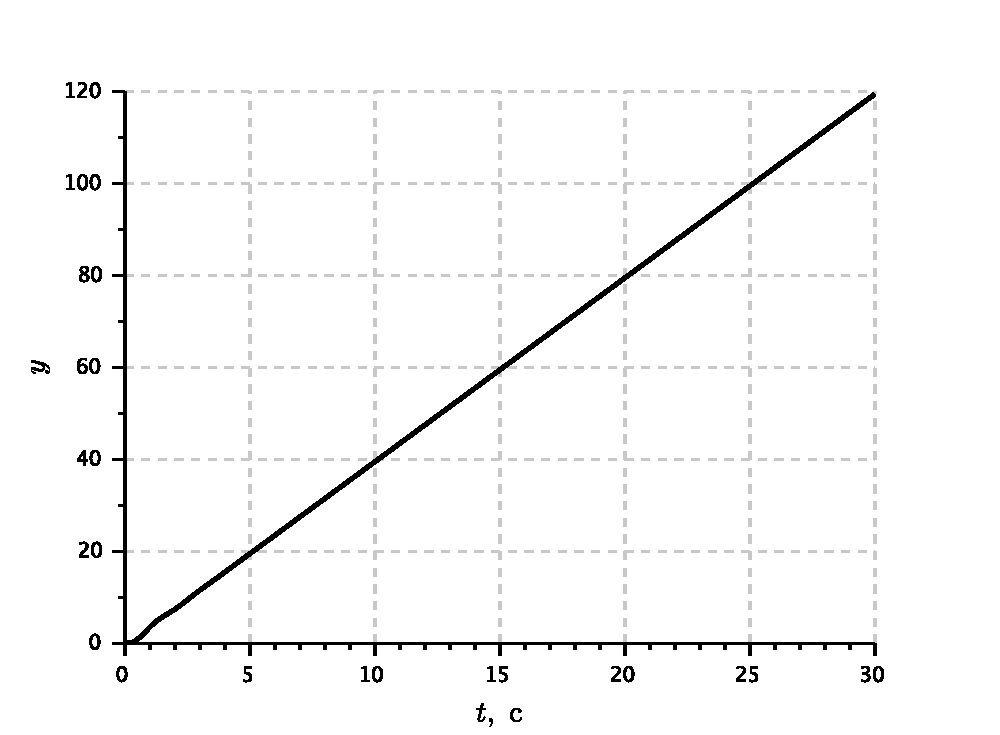
\includegraphics[width = \textwidth]{images/graph2-2-K5.pdf}
        \caption{k = 5}
    \end{subfigure}
    \begin{subfigure}{0.33\textwidth}
        \centering
        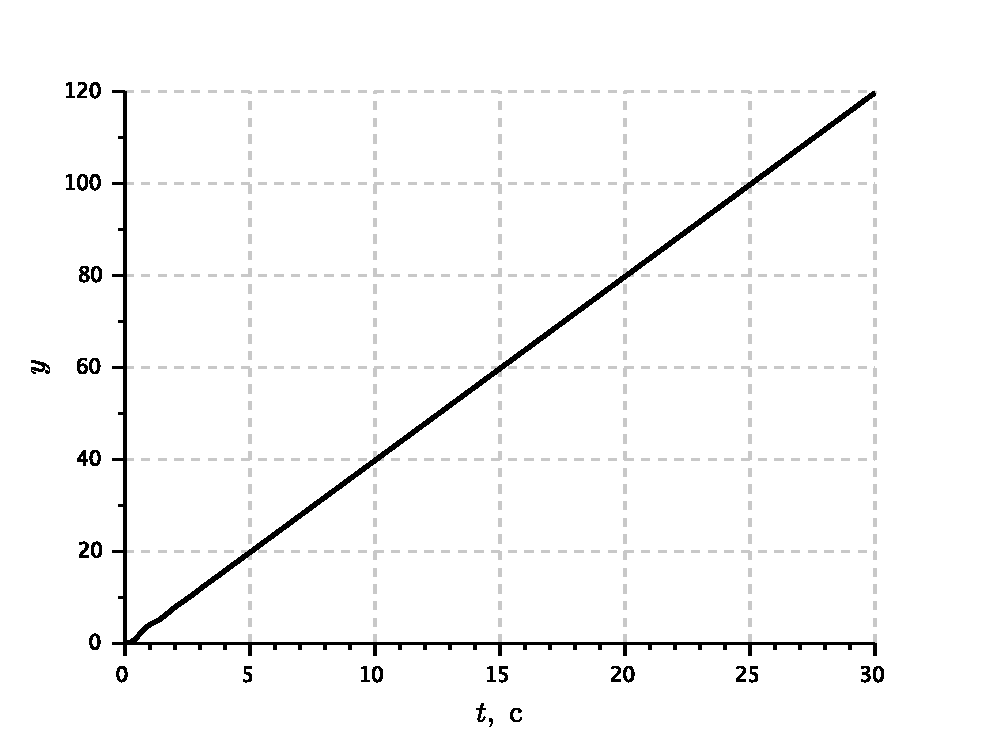
\includegraphics[width = \textwidth]{images/graph2-2-K10.pdf}
        \caption{k = 10}
    \end{subfigure}
    \caption{Графики при различных k.}
\end{figure}


\paragraph{Исследование движения с постоянным ускорением: $g(t) = 0.2t^2$.} На рисунках 9 и 10 представлены диаграмма модели и соответственно полученные графики при различных k.

\begin{figure}[h!]
    \centering
    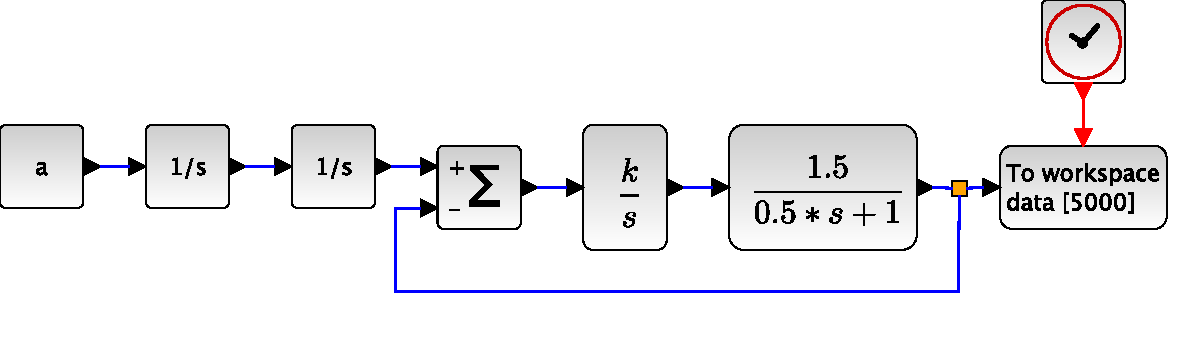
\includegraphics[width = 0.5\textwidth]{images/model2-3.pdf}
    \caption{Схема моделирования.}
\end{figure}

\begin{figure}[h!]
    \centering
    \begin{subfigure}{0.33\textwidth}
        \centering
        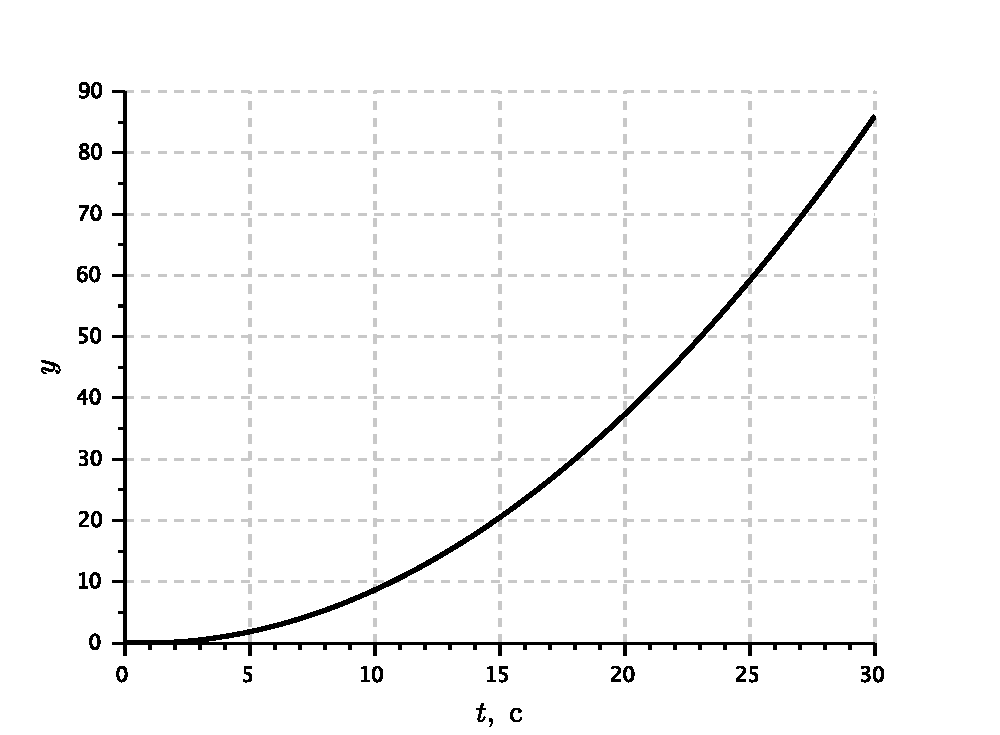
\includegraphics[width = \textwidth]{images/graph2-3-K1.pdf}
        \caption{k = 1}
    \end{subfigure}
    \begin{subfigure}{0.33\textwidth}
        \centering
        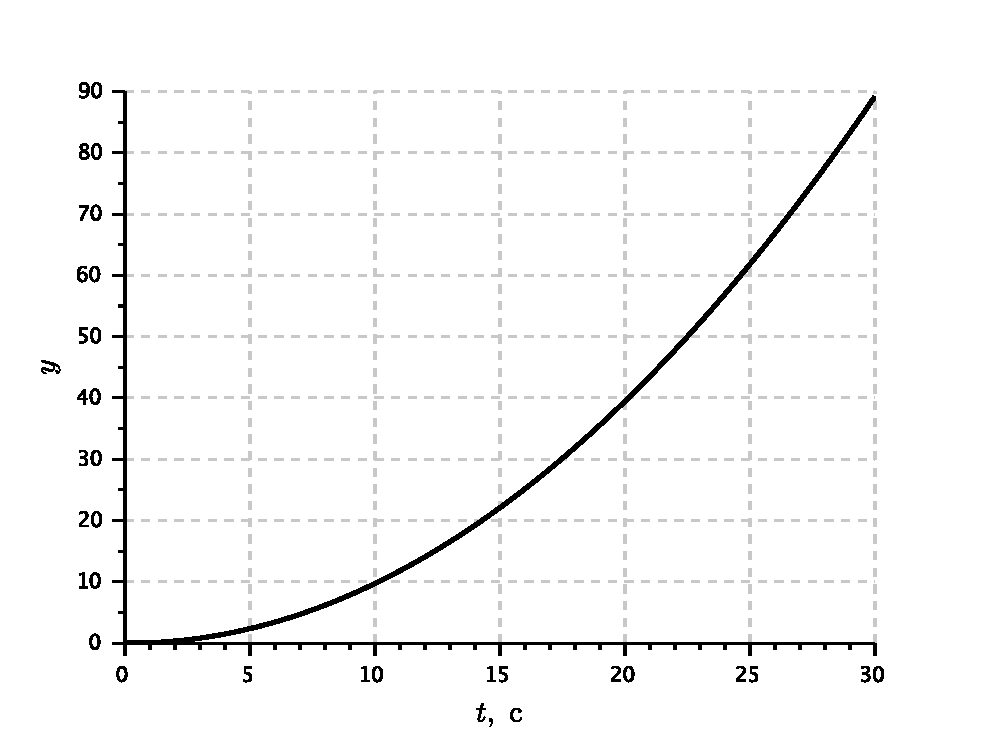
\includegraphics[width = \textwidth]{images/graph2-3-K5.pdf}
        \caption{k = 5}
    \end{subfigure}
    \begin{subfigure}{0.33\textwidth}
        \centering
        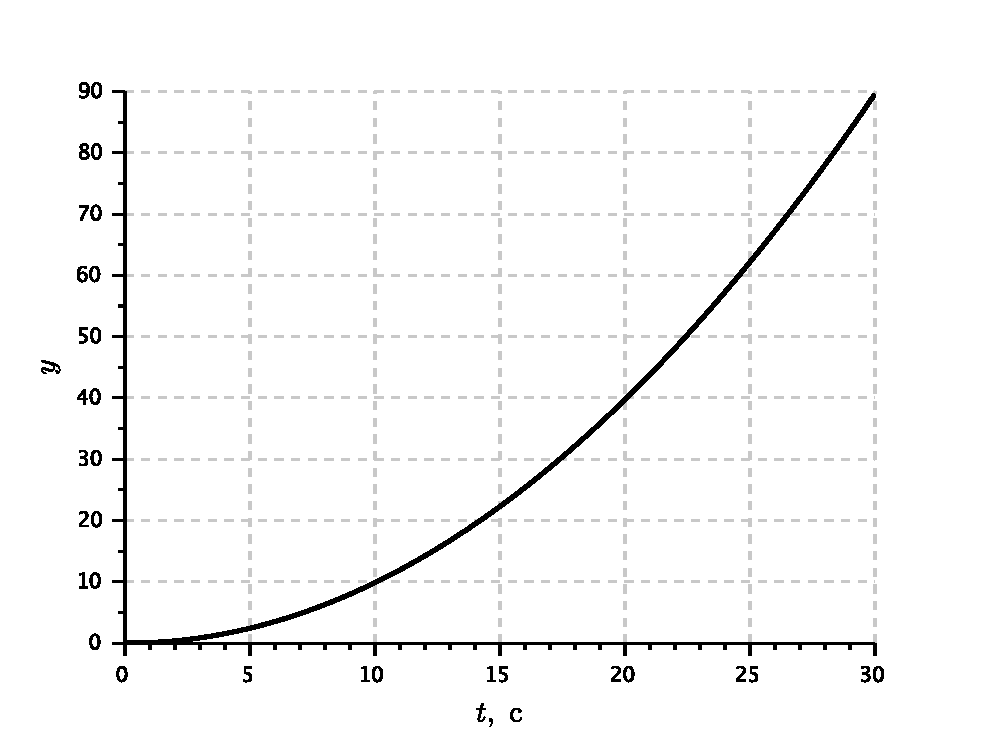
\includegraphics[width = \textwidth]{images/graph2-3-K10.pdf}
        \caption{k = 10}
    \end{subfigure}
    \caption{Графики при различных k.}
\end{figure}

\newpage

\section*{Исследование влияния внешних возмущений.}
На рисунках 11 и 12 представлены диаграмма модели и соответственно полученные графики при различных значениях шумов $f_1$ и $f_2$.

\begin{figure}[h!]
    \centering
    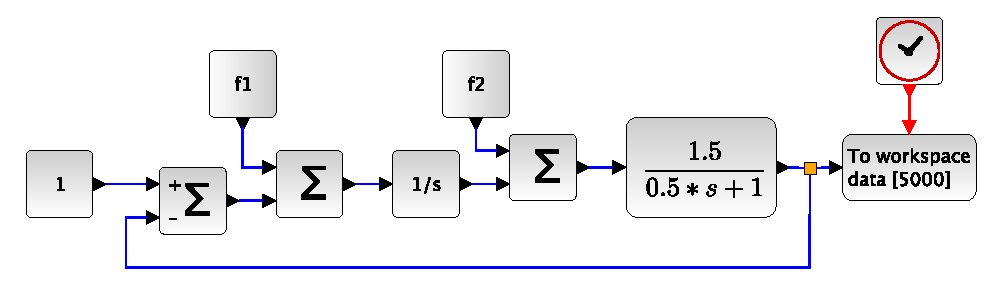
\includegraphics[width = 0.5\textwidth]{images/model3.pdf}
    \caption{Схема моделирования.}
\end{figure}
\begin{figure}[h!]
    \centering
    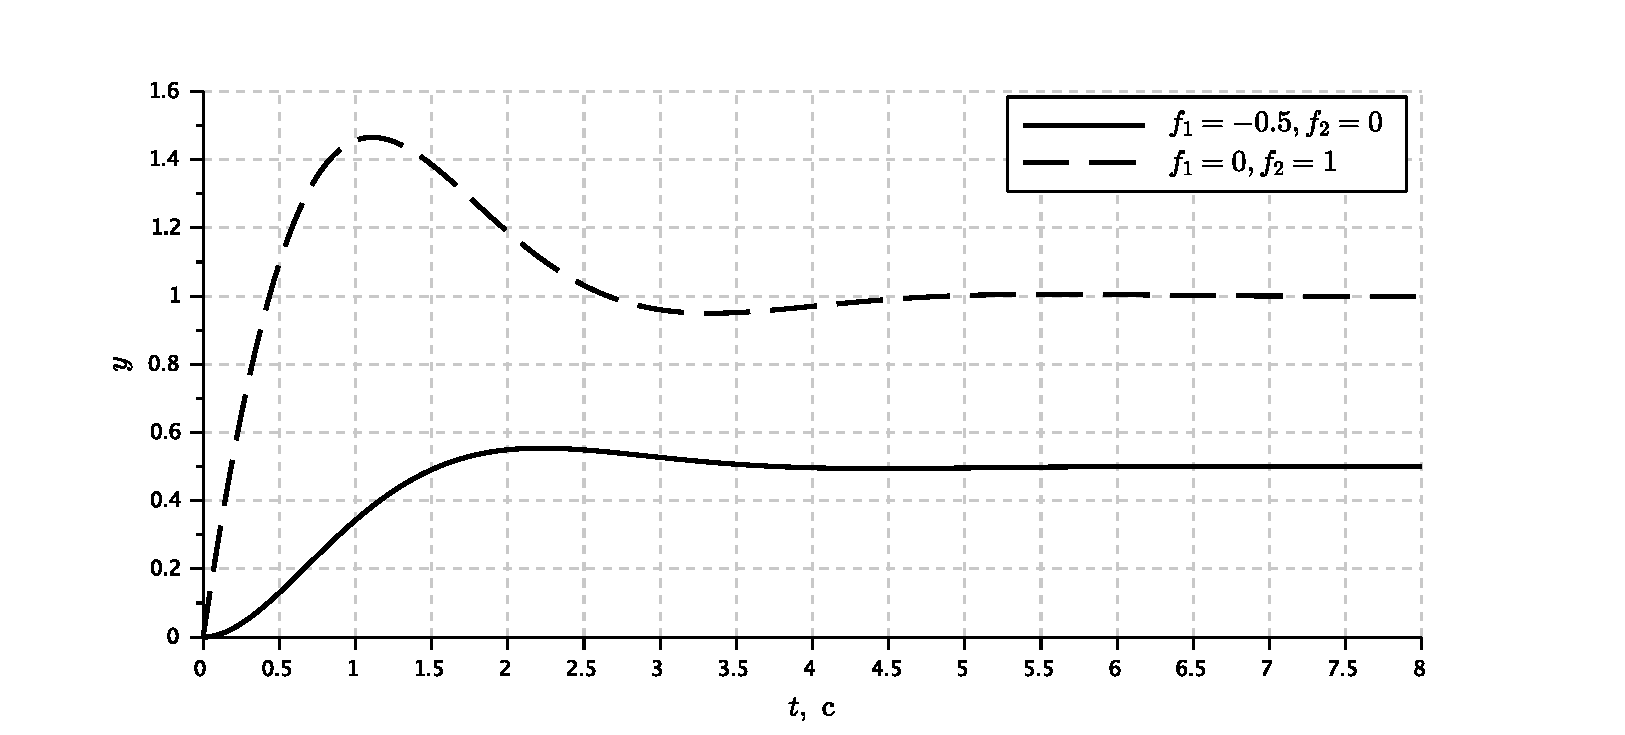
\includegraphics[width = 0.65\textwidth]{images/graph3.pdf}
    \caption{Графики при различных значениях шумов.}
\end{figure}

Функция ошибки в оператоном виде выглядить следущим образом:
\begin{equation}
    e(s) = \frac{g(0.5s^2 + s) - 1.5f_1 - 1.5f_2s}{0.5s^2 + s + 1.5}
\end{equation}
\par
Итак, при g = 2 можем записать выражения для предельного значения ошибки и подсчитать их значения при различных $f_1$ и $f_2$:
\begin{equation}
    \varepsilon = \lim_{s\rightarrow 0}{e(s)} = -f1;
\end{equation}
\begin{align*}
    \varepsilon|_{f_1 = -0.5, f_2 = 0.5} & = 0.5 & \varepsilon|_{f_1 = 0, f_2 = 1} & = 0
\end{align*}

\section*{Исследование установившейся ошибки при произвольном входном воздействии.}
На рисунках 13 и 14 представлены диаграмма модели и соответственно полученные графики при различных значениях шумов $f_1$ и $f_2$.

\begin{figure}[h!]
    \centering
    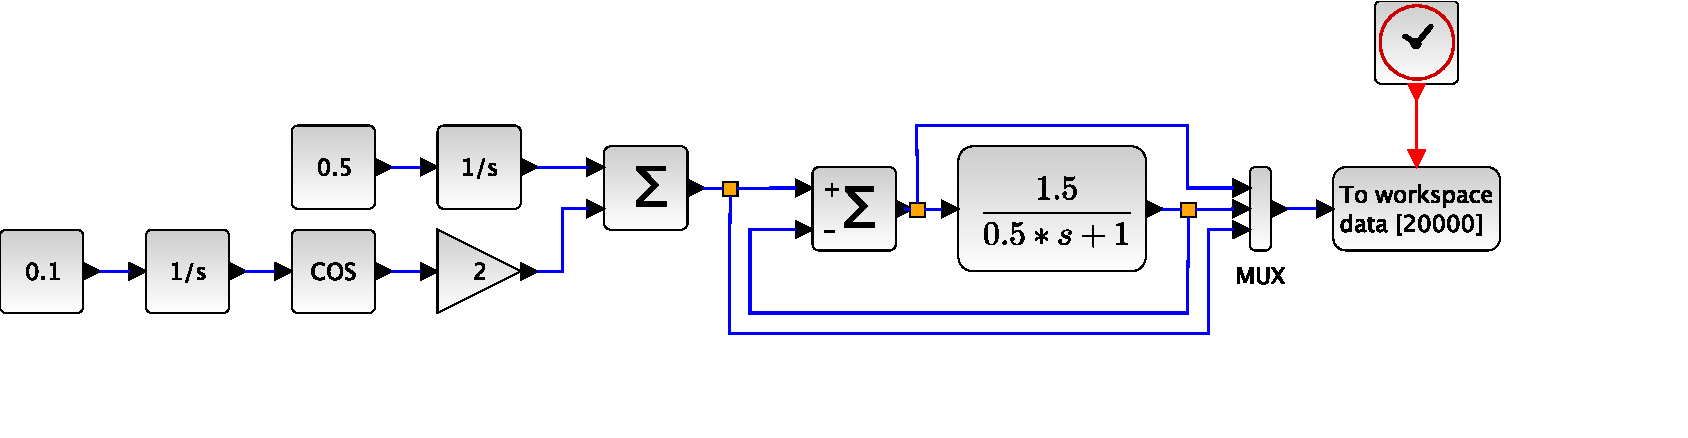
\includegraphics[width = 0.7\textwidth]{images/model4.pdf}
    \caption{Схема моделирования.}
\end{figure}
\begin{figure}[h!]
    \centering
    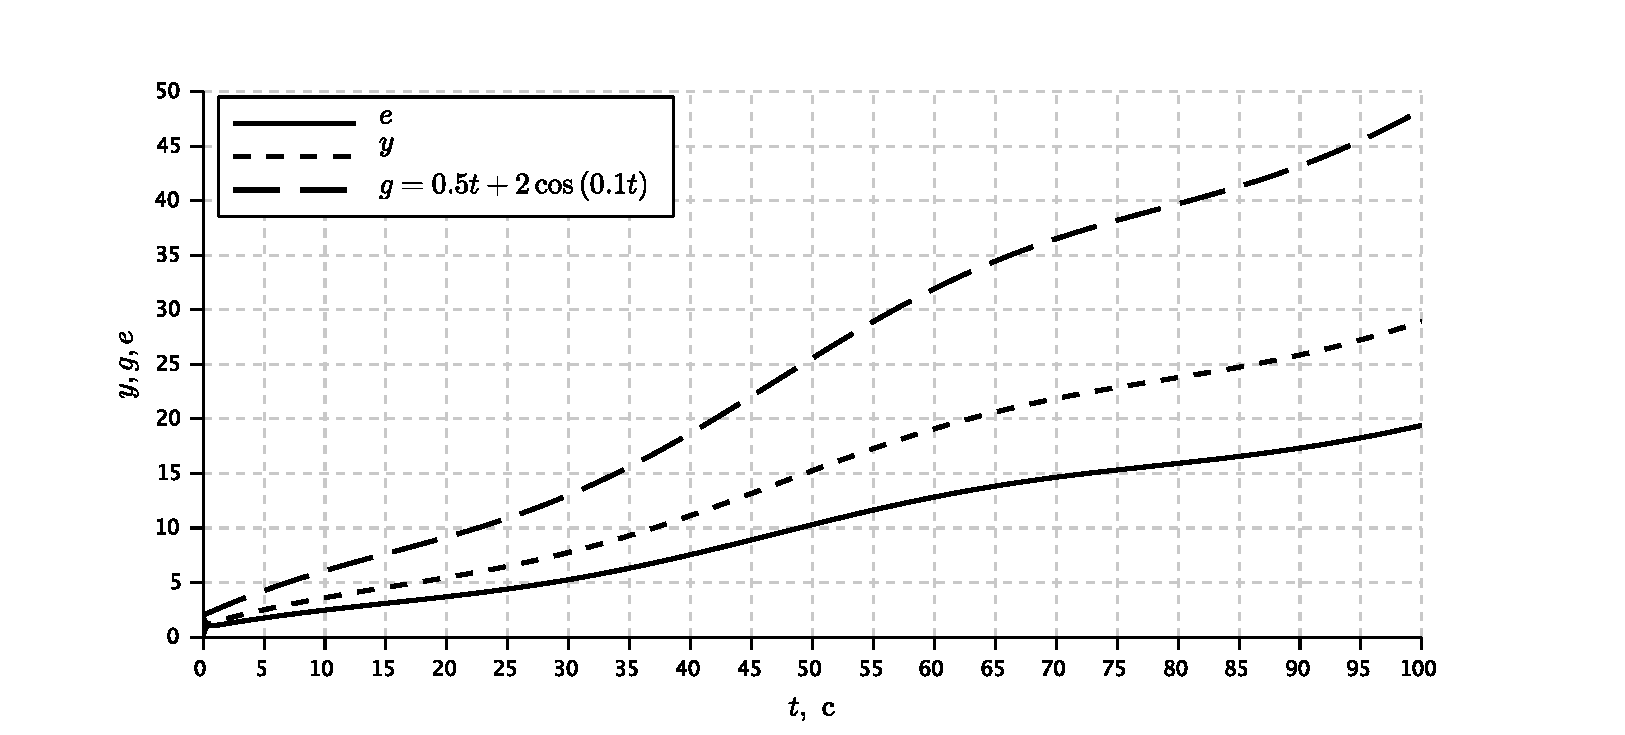
\includegraphics[width = 0.65\textwidth]{images/graph4.pdf}
    \caption{Графики ошибки, выходного и входного сигнала.} 
\end{figure}

Как видно из графика ошибки (рисунок 14) она представлена уравнением с постоянно возрастающей и гармонической составляющей. Ее вид можно записать следующим образом: 
\begin{equation}
    e(t) = at + b + c\sin{(0.1t + \varphi_0)}
\end{equation}
\par
Здесь $at + b$ задает уравнение прямой, и $c\sin{(0.1 + \varphi_0)}$ описывает гармонические колебание вдоль этой прямой. Теперь давайте найдем коэффициенты и элементы разложенной в ряд Тейлора уравнения ошибки. Само разложение (до третьего члена) выглядит следующим образом. 
\begin{equation}
    e(t) = W_e(s)|_{s\rightarrow0}g(t) + \left.\frac{dW_e(s)}{ds}\right|_{s\rightarrow0}\dot{g}(t) + \left.\frac{d^2W_e(s)}{ds^2}\right|_{s\rightarrow0}\frac{\ddot{g}(t)}{2!}
\end{equation}

Для это необходимо взять производные по задающиму воздействию, а также передаточной функции ошибки. Они задаются уравнениями: 

\begin{align}
    W_{e}(s) & = \frac{0.5s + 1}{0.5s + 2.5} \\ 
    g(t) & = 0.5t + 2\cos{(0.1t)}
\end{align}
\par

Производные:
\begin{align*}
    g(t) & & W_e(s)|_{s\rightarrow0} & = 0.4 \\
    \dot{g}(t) & = 0.5 - 0.2\sin{(0.1t)} & \left.\frac{dW_e(s)}{ds}\right|_{s\rightarrow0} & = 0.12 \\
    \ddot{g}(t) & = -0.02\cos{(0.1t)} & \left.\frac{d^2W_e(s)}{ds^2}\right|_{s\rightarrow0} & = -0.048 \\
\end{align*}
\par

Подставив полученные значения в уравнение (8) получим искомое выражение для ошибки.
\begin{equation}
    e(t) = 0.2t + 0.06 + 0.80048\cos{(0.1t)} - 0.024\sin{0.1t}
\end{equation}
\par
Теперь можем получить графики ошибки, разложенной в ряд и реальной.
\begin{figure}[h!]
    \centering
    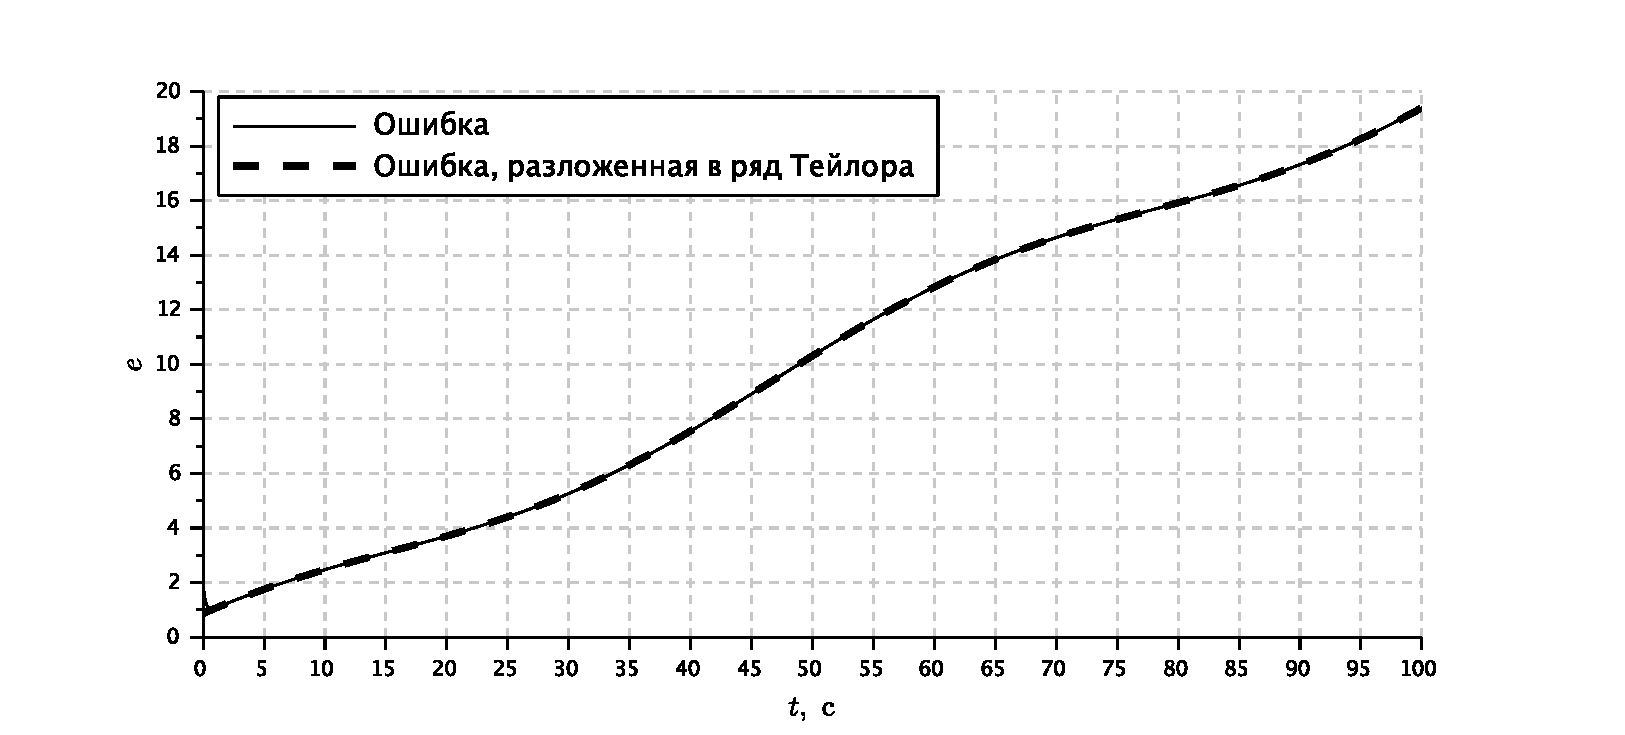
\includegraphics[width = 0.8\textwidth]{images/graph4withTailor.pdf}
    \caption{Графики ошибок.}
\end{figure}


\section*{Выводы.}
В данной работе мы исследновали системы с различным астатизмом, при налчии внешних возмущений и при произвольно входном воздействии. Получили значения и выражение для предельного значения установившейся ошибки и построили графики переходной характеристики. \par
При исследовании стационарного режима работы, убедились в том, что при g = A, и увеличении коэффициента усиления k ошибка стремиться к нулю. 
Убедились в том, что при увеличении прядка астатизма, ошибка, при статическом вохдном возвдействии ошибка равна нулю.
Внешние возмущения могут оказвать довольно сильное влияние - изменение выходного сигнала в 2 раза, сильное перерегулироване.
\end{document}
